\documentclass[../main.tex]{subfiles}
\graphicspath{{\subfix{../media/}}}


\begin{document}
	\begin{figure}[h]
		\centering
	    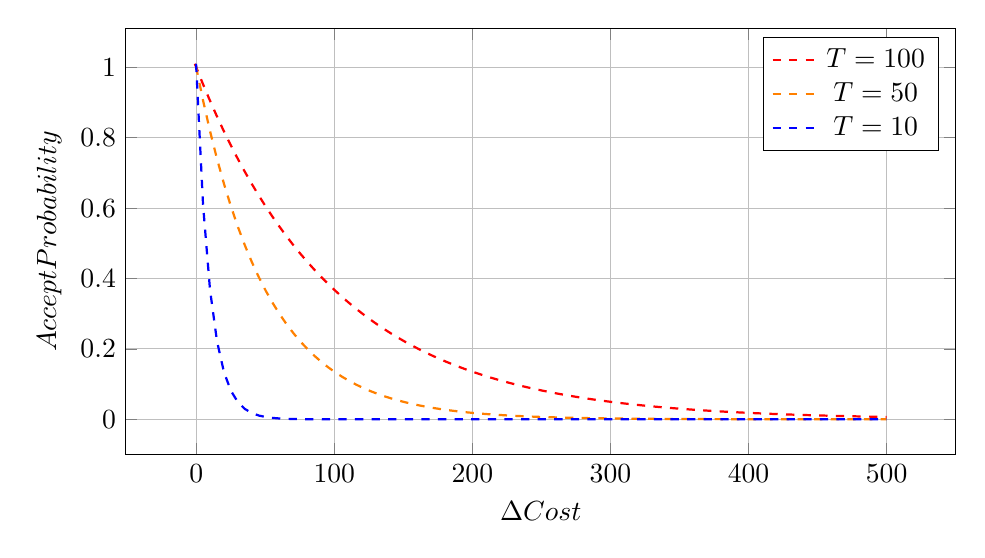
\begin{tikzpicture}
	        \begin{axis}[
	            xlabel = $\Delta \text{Cost}$,
	            ylabel = $\text{Accept Probability}$,
			  	width=\linewidth,
			  	height=7cm,
			  	grid=both,
	            declare function={
	                l0(\cost) = exp(-\cost/100);
	                l1(\cost) = exp(-\cost/10);
	            }
	        ]
	            
	            % Bases Functions
	            \addplot[thick, dashed, red, domain=-1:500, samples=100] {exp(-\x/100)};
	            \addplot[thick, dashed, orange, domain=-0.1:500, samples=100] {exp(-\x/50)};
	            \addplot[thick, dashed, blue, domain=-0.1:500, samples=100] {exp(-\x/10)};
					            
				\legend{$T=100$ , $T=50$, $T=10$}

	        \end{axis}
	    \end{tikzpicture}
	    \caption{Simulated Annealing Temperature }
	\end{figure}

\end{document}